%++++++++++++++++++++++++++++++++++++++++
% Don't modify this section unless you know what you're doing!
\documentclass[letterpaper,12pt]{article}
\usepackage{tabularx} % extra features for tabular environment
\usepackage{amsmath}  % improve math presentation
\usepackage{graphicx} % takes care of graphic including machinery
\usepackage[margin=1in,letterpaper]{geometry} % decreases margins
\usepackage{cite} % takes care of citations
\usepackage[final]{hyperref} % adds hyper links inside the generated pdf file
\usepackage{kotex}
\hypersetup{
	colorlinks=true,       % false: boxed links; true: colored links
	linkcolor=blue,        % color of internal links
	citecolor=blue,        % color of links to bibliography
	filecolor=magenta,     % color of file links
	urlcolor=blue         
}
%++++++++++++++++++++++++++++++++++++++++


\begin{document}

\title{GIT 사용법}
\author{20142503 백찬희}
\date{\today}
\maketitle

\section{GIT이란?}

버전관리 시스템 중 하나로 파일 변화를 시간에 따라 버전으로 기록했다가 나중에 특정 시점의 버전을 다시 꺼내올 수 있는 시스템이다. 
저장한 버전들을 이용해 파일을 이전 상태로 되돌리거나 시간에 따라 수정 내용을 비교하거나 누가 문제를 일으켰는지 누가 언제 만들었는지 등을 알 수 있다. 


\section{설치방법}

\href{https://git-scm.com/}{https://git-scm.com/}에서 해당하는 \textit{OS}에 맞게 설치를 한다. 설치 파일 중 \textbf{git bash}를 이용하면 \textit{Windows}에서 \textit{Linux}, \textit{MacOS}와 같은 환경에서 \textbf{GIT}을 사용할 수 있다. 아래에 적혀있는 모든 명령어는 \textbf{git bash}에서 작성한 것이다.

\section{GIT 초기설정}

버전관리를 원하는 프로젝트 디렉토리 들어간 뒤 다음과 같은 명령어를 입력한다.
\begin{verbatim}
git init
\end{verbatim} 
위의 명령어를 통해 현재 디렉토리가 버전관리 되는 저장소로 선언한 것이다.
\\\\만약 이미 \textit{github.com}과 같은 원격저장소가 이미 존재하는 경우에는 다음 명령어를 통해 로컬저장소로 파일들을 그대로 가져올수 있다.
\begin{verbatim}
git clone 해당URL
\end{verbatim} 
버전관리를 시작하기 전 먼저 사용자 정보를 설정해야 한다. 
\begin{verbatim}
git config --global user.name 해당이름
git config --global user.email 해당이메일
\end{verbatim} 
이를 통해 버전마다 누가 작성했는지 알 수 있다.

\clearpage

\begin{figure}[ht] 
        % read manual to see what [ht] means and for other possible options
        \centering 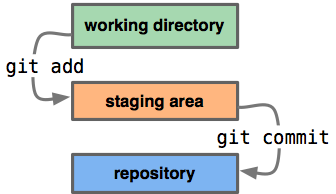
\includegraphics[width=0.8\columnwidth]{git}
        % note that in above figure file name, "sr_setup",
        % the file extension is missing. LaTeX is smart enough to find
        % apropriate one (i.e. pdf, png, etc.)
        % You can add this extention yourself as it seen below
        % both notations are correct but above has more flexibility
        %\includegraphics[width=1.0\columnwidth]{sr_setup.pdf}
         \caption{
                \label{fig:git}  
                7.GIT의 원리에서 더 자세히 설명
        }
\end{figure}
\section{버전 만들기}
버전을 만들기 위해서는 버전관리의 대상으로 설정하고 싶은 파일들을 다음 명령으로 \textbf{staging area}(그림 참고)에 올린다.
\begin{verbatim}
git add 파일명
\end{verbatim}
프로젝트 디렉토리(working directory)에 다음과 같이 파일이 있다 가정하고 \textit{git add 파일1} 을 했을시 다음과 같다.
\begin{table}[ht]
\begin{center}
\label{tbl:bins} % spaces are big no-no withing labels
\begin{tabular}{|ccc|} 
\hline
\multicolumn{1}{|c}{working directory} & \multicolumn{1}{c}{staging area} & repository\\
\hline
파일1 &   파일1 & \\
파일2 &    & \\
파일3 &    & \\
파일4 &    & \\
\hline
\end{tabular}
\end{center}
\caption{git add 파일1}
\end{table}
\\이 상태에서 다음 명령을 내리면 staging area 올라온 파일들을 사진을 찍듯이 현재상황 그대로 버전으로 등록을 한다. 
\begin{verbatim}
git commit -m "버전을 설명하는 문구"
\end{verbatim}

\clearpage

\begin{table}[ht]
\begin{center}
\label{tbl:bins} % spaces are big no-no withing labels
\begin{tabular}{|ccc|} 
\hline
\multicolumn{1}{|c}{working directory} & \multicolumn{1}{c}{staging area} & repository\\
\hline
파일1 &   파일1 & 버전1(파일1)\\
파일2 &    & \\
파일3 &    & \\
파일4 &    & \\
\hline
\end{tabular}
\end{center}
\caption{git commit}
\end{table}
만약 파일1을 수정하고 이를 다음 버전에 등록하고 싶다면 반드시 다시 staging area에 올리는 명령을 실행해야 한다. 
\begin{verbatim}
git add 파일1
\end{verbatim}

\begin{table}[ht]
\begin{center}
\label{tbl:bins} % spaces are big no-no withing labels
\begin{tabular}{|ccc|} 
\hline
\multicolumn{1}{|c}{working directory} & \multicolumn{1}{c}{staging area} & repository\\
\hline
파일1* &   파일1 & 버전1(파일1)\\
파일2 &    & \\
파일3 &    & \\
파일4 &    & \\
\hline
\end{tabular}
\end{center}
\caption{파일1을 수정하고 add 하기 전}
\end{table}

\begin{table}[ht]
\begin{center}
\label{tbl:bins} % spaces are big no-no withing labels
\begin{tabular}{|ccc|} 
\hline
\multicolumn{1}{|c}{working directory} & \multicolumn{1}{c}{staging area} & repository\\
\hline
파일1* &   파일1* & 버전1(파일1)\\
파일2 &    & \\
파일3 &    & \\
파일4 &    & \\
\hline
\end{tabular}
\end{center}
\caption{git add 파일1 한 이후}
\end{table}

다음 버전을 만들기 전에 파일2도 staging area에 올리는 상황을 가정한다.

\clearpage

\begin{table}[ht]
\begin{center}
\label{tbl:bins} % spaces are big no-no withing labels
\begin{tabular}{|ccc|} 
\hline
\multicolumn{1}{|c}{working directory} & \multicolumn{1}{c}{staging area} & repository\\
\hline
파일1* &   파일1* & 버전1(파일1)\\
파일2 &    파일2& \\
파일3 &    & \\
파일4 &    & \\
\hline
\end{tabular}
\end{center}
\caption{git add 파일2}
\end{table}

이 상태에서 commit을 하면 앞에서 봤듯이 staging area의 상황을 사진으로 찍는 것처럼 repository에 버전으로 등록을 한다.

\begin{table}[ht]
\begin{center}
\label{tbl:bins} % spaces are big no-no withing labels
\begin{tabular}{|ccc|} 
\hline
\multicolumn{1}{|c}{working directory} & \multicolumn{1}{c}{staging area} & repository\\
\hline
파일1* &   파일1* & 버전1(파일1)\\
파일2 &    파일2& 버전2(파일1*,파일2)\\
파일3 &    & \\
파일4 &    & \\
\hline
\end{tabular}
\end{center}
\caption{git commit}
\end{table}

다음과 같이 commit을 할 때마다 버전이 하나씩 만들어 진다.
\section{버전 간의 차이 보기}
버전들을 저장해서 얻는 유용한 점들 중 하나가 버전 간의 차이를 볼 수 있다는 점이다.
\\\\ 다음 명령은 지금까지의 버전 정보들(log)을 보여주고 인접한 버전들간의 차이점을 보여주는 명령이다.
\begin{verbatim}
git log -p
\end{verbatim}
버전마다 고유한 해쉬값이 존재한다. 다음 명령은 비교하고자 하는 두 버전의 해쉬값을 이용해 차이점을 보여주는 명령이다. 
\begin{verbatim}
git diff '버전1해쉬값'..'버전2해쉬값'
\end{verbatim}
다음 명령은 버전들 간의 차이점을 보여주는 명령이 아니다. working directory에 있는 파일 중 staging area에 올라가 있는 파일\textit{(Table 6 기준: 파일1, 파일2)}을 수정했지만 staging area에 등록하지 않았을 경우 staging area에 있는 파일과 변경된 working directory에 있는 파일을 비교해 보여주는 명령이다. 쉽게 예를 들면 Table 3에서 파일1* 과 파일1의 차이점을 보여주는 명령이다.
\begin{verbatim}
git diff
\end{verbatim}
다음 명령은 staging area에 있는 파일과 repository에서 가장 최신 버전에 있는 파일들을 비교하는 명령이다.
\begin{verbatim}
git diff --cached
\end{verbatim}


\section{과거의 버전으로 되돌아가기}
버전들을 저장해서 얻는 유용한 점들 중 또다른 하나는 현재 버전에 문제가 발생했을 경우 과거의 버전으로 되돌아 갈 수 있다는 점이다.
\\\\다음 명령은 돌아가고 싶은 버전의 해쉬값으로 이동하는데 이 버전보다 최신이었던 버전들은 삭제가 되는 방식이다.
\begin{verbatim}
git reset '버전해쉬값'
\end{verbatim}
예를 들어 버전1 - 버전2 - 버전3 - 버전4 가 있다고 가정하자. git reset '버전2해쉬값'을 하면 repository에 버전1 - 버전2만 남아있고 버전2가 가장 최신 버전이 된다.
\\\\
다음 명령은 돌아가고 싶은 버전의 해쉬값을 입력하면 앞의 명령과는 다르게 버전들이 삭제가 되지 않고 돌아가고 싶은 버전보다 최신이었던 버전들의 내용이 반영되지 않는 새로운 버전을 만들어 낸다.  
\begin{verbatim}
git revert '버전해쉬값'
\end{verbatim}
예를 들어 버전1 - 버전2 - 버전3 - 버전4 가 있다고 가정하자. git revert '버전2해쉬값'을 하면 repository에 버전1 - 버전2 - 버전3 - 버전4 - 버전5가 만들어진다. 버전5는 버전3, 버전4의 변경사항을 반영하지 않는 새로운 버전이다.

\section{GIT의 원리}
Figure 1에 있는 \textbf{working directory}, \textbf{staging area}, \textbf{repository}가 실제로 어떤 것인지 알아보겠다.
\\\\\textbf{working directory}는 git init을 했던 프로젝트 디렉토리이다. 프로젝트 파일을 생성, 수정을 하면 working directory에서만 반영되는 것이다. git add을 해야 staging area에 올라가 버전에 등록할 수 있다. 
\\심지어 프로젝트 파일을 삭제하면 working directory에서 바로 삭제가 이루어지지만, staging area와 repository에는 파일이 그대로 남아있다. \\만약 working directory와 staging area가 구분되지 않았더라면 불필요한 파일까지 버전관리가 되는 상황이 발생하기 때문에 이처럼 분리를 했다.
\clearpage
\textbf{staging area}는 git init을 했을 때 생성된 \textit{.git} 디렉토리 내부 \textit{index} 파일을 나타내는 것이다. index 파일 내부에는 git add를 한 파일만 등록이 이루어진다. \\index 파일에 파일의 내용이 직접 저장되는 것이 아니라 파일의 내용을 SHA-1 해쉬함수를 거쳐 해쉬값들의 목록을 저장한다. \\해쉬함수는 일방향 함수로 파일의 내용이 같으면 똑같은 해쉬값을 출력한다. 따라서 파일의 내용이 같으면 해쉬값도 같기 때문에 변경이 없다는 것을 알 수 있고 파일의 내용이 달라지면 해쉬값 또한 달리지기 때문에 변경이 있다는 것을 알 수 있다. \\ 실제 파일은 blob object 형태로 저장되며 해쉬값을 주소처럼 이용해 해당 object를 쉽게 찾을 수 있다.
\begin{figure}[ht] 
        % read manual to see what [ht] means and for other possible options
        \centering 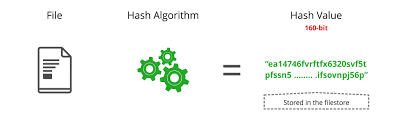
\includegraphics[width=0.8\columnwidth]{hash}
        % note that in above figure file name, "sr_setup",
        % the file extension is missing. LaTeX is smart enough to find
        % apropriate one (i.e. pdf, png, etc.)
        % You can add this extention yourself as it seen below
        % both notations are correct but above has more flexibility
        %\includegraphics[width=1.0\columnwidth]{sr_setup.pdf}
         \caption{
                \label{fig:hash}  
                모든 object마다 hash값을 구할 수 있다.
        }
\end{figure}

\textbf{repository}는 commit object 형태로 존재한다. commit object에는 commit한 사람의 정보, commit할 때 남긴 메시지, 이전 버전의 commit object 해쉬값, blob object들의 해쉬값 목록을 모아둔 tree object의 해쉬값으로 구성된다. 아래 그림과 같이 체인처럼 버전들이 연결 되어 있다.
\begin{figure}[ht] 
        % read manual to see what [ht] means and for other possible options
        \centering 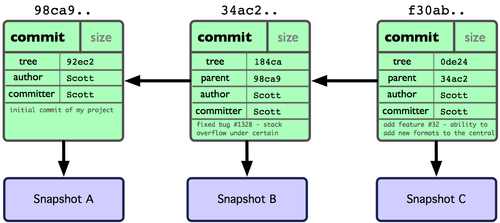
\includegraphics[width=0.8\columnwidth]{repository}
        % note that in above figure file name, "sr_setup",
        % the file extension is missing. LaTeX is smart enough to find
        % apropriate one (i.e. pdf, png, etc.)
        % You can add this extention yourself as it seen below
        % both notations are correct but above has more flexibility
        %\includegraphics[width=1.0\columnwidth]{sr_setup.pdf}
         \caption{
                \label{fig:repository}  
                repository
        }
\end{figure}

\section{원격저장소와 동기화하기}
원격저장소는 소스코드와 버전을 백업하고, 다른 사람과 협업을 하기 위한 핵심적인 기능이다. 원격저장소로 정말 유명한 \textbf{Github}말고도 내 컴퓨터의 다른 드라이브를 원격저장소로 사용할 수 있고 서버컴퓨터를 원격저장소로 사용할 수도 있다. 하지만 그 중에서 Github에 원격저장소를 만들고 지역저장소에 있는 파일들을 올려보겠다.   

















\begin{thebibliography}{99}

\bibitem{melissinos}
A.~C. Melissinos and J. Napolitano, \textit{Experiments in Modern Physics},
(Academic Press, New York, 2003).

\bibitem{Cyr}
N.\ Cyr, M.\ T$\hat{e}$tu, and M.\ Breton,
% "All-optical microwave frequency standard: a proposal,"
IEEE Trans.\ Instrum.\ Meas.\ \textbf{42}, 640 (1993).

\bibitem{Wiki} \emph{Expected value},  available at
\texttt{http://en.wikipedia.org/wiki/Expected\_value}.

\end{thebibliography}


\end{document}
